% !TEX root =/main.tex
\chapter{Exam 1}
\section{Q1 - 15p}
\renewcommand{\thesubsection}{\alph{subsection}}
\subsection{1p}
In what way does shared mutable data cause a problem in parallel programming?

When parallel processes read and edit the same data range, it's very common to run into issues that one process overwrites what the other has done.

\subsection{1p}
Haskell sparks and the libraries we build using them (for example Strategies) give us deterministic parallelism. What do we mean by this?

If we in several different parts of a program calls a function with the same input, we will get the same output every time, meaning if all of those function calls are sparked, as soon as one of them are calculated, we can kill the other sparks and use that result everywhere.

\subsection{1p}
Compare the \textit{Strategies} and \textit{Par} monad approaches to parallel programming in Haskell. In what ways do they differ?

---------------------

\subsection{1p}
If we have a Haskell strategy $s$ and a value $v$, we can evaluate the value using the strategy by writing $v$ 'using' $s$. Can we say that the law $v$ 'using' $s == v$ holds? If not, why might it not hold?


Yes, strategies define in which way we parallelize the execution, not what the execution will result in, meaning, while the time to execute the two things is different, the resulting value is the same (except for the monadicness of the strategized value).

\subsection{1p}
''After parallelization, any program should be able to run $N$ times faster on $N$ cores.'' Is this true or false? Explain your answer briefly (for example, with reference to \textit{Amdahl's Law}).

This is not true, Amdahl's Law recognizes that certain parts of every program can't be parallelized, for example when writing to disk. If we for example write a hello world-program it doesn't help the execution to use 2000 cores, with that many cores we might be able to write to lots of screens, but the time to write to a single screen will not decrease.

\subsection{1p}
To parallelise reduce or scan, we must assume that the binary operator is associative. Explain why this is.

-------------------------

\subsection{1p}
Do parallel processes share memory in
\begin{enumerate}[i]
	\item Haskell?
	      \subitem Yes, but since functions have no side effects it doesn't matter if the same address is written to twice
	\item Erlang?
	      \subitem  No, each process has its own memory allocated to it.
\end{enumerate}

\subsection{1p}
Control of granularity is important in parallel programming. Why is this? Briefly explain two ways in which you have controlled granularity in your programs, one in Haskell and one in Erlang.



\subsection{1p}
Haskell and Erlang both use \textit{garbage collection} to recycle memory, but they work rather differently. What aspect of garbage collection may cause a problem in real-time systems, and how does Erlang's VM design mitigate that problem?



\subsection{1p}
After an Erlang process sends a message using \lstinline{Pid ! Msg,} does the sending process continue its execution \begin{enumerate}[i]
\item immediately,
\item once the message is safely delivered to the recipient's mailbox,
\item once the recipient has \lstinline{receive}d the message from its mailbox,
\item once the recipient has sent a reply?
\end{enumerate}

immediately

\subsection{1p}
What do Erlang developers mean by ''\textit{Let it crash}'', and why do they consider it a good idea?

Since the resources of each process in Erlang is independent and the ease of creating new processes, it's often smarter to abandon a faulty process and start a new one, instead of trying to work with a potentially faulty one.

\subsection{1p}
What is the purpose of a supervisor?

A supervisor are used to make sure tasks are assigned to processes effectively and to handle what happens when a process fails and crashes.

\subsection{1p}
''Modern networks are so fast that placement of processes on machines is not important.'' In the context of Erlang, is this true or false? Explain your answer.

It makes a difference if everything is on a machine or spread across several

\subsection{1p}
What is \textit{speculative parallelism} and how might it be used in a search algorithm?

Speculative parallelism is similar to speculative execution, if it takes a long time to evaluate which path a process should execute in e.g. an if-statement, both paths might start to be executed in parallel while waiting for which one is correct. If we search for something, this means we can start searching several branches before knowing which one is the correct, leading to faster execution.

\subsection{1p}
Why can speculative parallelism lead to poor overall performance? How would you prevent this from happening?

It can be very resource intensive to search a lot of unnecessary branches, if this is a problem we can make sure to not evaluate as much before knowing which path is correct.

\section{Q2 - 4p}
\begin{figure}[H]
	\centering
	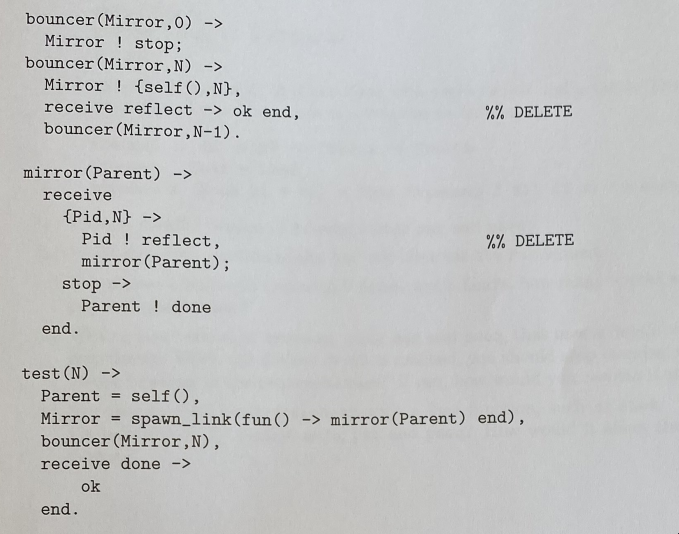
\includegraphics[width=0.7\textwidth]{images/24_2.png}
	\label{fig:24_2}
	\caption{Study the benchmark code above}
\end{figure}
The function \lstinline{test} starts a 'mirror' process, that replies to every message with the reply \lstinline{reflect}, until it receives an instruction to \lstinline{stop}, then \lstinline{test} runs a 'bouncer' that sends N messages to the mirror, then tells it to stop. By calling, for example \lstinline{test(100)} we can benchmark message parsing in Erlang.
This benchmark shows that the two processes could exchange around a million message pairs a second.
\subsection{2p}
If we were to \textit{remove} the two lines marked \lstinline{DELETE}, so that the mirror did not send replies to the bouncer, and run the same test (on a multicore computer), would you expect it to take roughly
\begin{enumerate}[i]
	\item the same amount of time
	\item half the time
	\item one quarter the time
	\item considerably less than one quarter the time
\end{enumerate}
Why?

\textbf{Answer: } Without the receive and mirror's send, the execution time would run in considerably less than one quarter of the time.Without that, the program is little more than a for-loop.

\subsection{2p}
If the mirror process were run on a different computer, so that communication took place over a network rather than within one virtual machine, then of course the test would run more slowly. But how would the relative performance of the two versions of the test be affected? Choose one answer below and explain your reasons.
\begin{enumerate}[i]
	\item Both versions of the test would run slower, but the ratio between the time taken with and without reflect messages would be about the same as on a single computer.
	\item Both versions of the test would run slower, but because communication time dominates computation time, then the difference in performance between the tests with and without reflect messages would not be significant.
	\item Both versions of the test would run slower, but the tests with reflect messages would be much worse affected than those without.
\end{enumerate}
The last one is true, if the time it takes to receive a message is higher, the version where we have to wait for a response before sending the next message will take considerably more time.

\section{3 - 11p}
Consider the definition of a binary tree below
\begin{lstlisting}{ha}
	data Tree a
	= Node (Tree a) a (Tree a)
	| Leaf
\end{lstlisting}
A tree is either a Leaf, or it is a Node with two subtrees and a value. The function that maps a transformation over the values of a tree can be written as \begin{lstlisting}
	treemap :: (a-> b) -> Tree a -> Tree b
	treemap _ Leaf = Leaf
	treemap f (Node t1 v t2) = Node treemap f t1 (f v) (treemap f t2)
\end{lstlisting}
\subsection{3p}
Write a parallel version of treemap using par and pseq.

\begin{lstlisting}
	treemap' :: (a -> b) -> Tree a -> Tree b
	treemap _ Leaf = Leaf
	treemap f (Node l v r) = do
		let x =(treemap f' l)
		let y = (treemap f' r)
		let vv = (f v)
		par Node (pseq x (pseq vv y))
\end{lstlisting}

\subsection{3p}
Write the same function again, but this time use the Par monad.

\begin{lstlisting}
	treemap _ Leaf = Leaf
	treemap f (Node l v r) = runPar $ do
		x' <- spawn (treemap f' l)
		y' <- spawn (treemap f' r)
		vv <- return  (f v)
		x <- get x'
		y <- get y'
		return Node x vv y
\end{lstlisting}

\subsection{1p}
If you have a balanced tree with 7 Nodes and 8 Leafs, how many sparks will your function using par and pseq create?
14?

\subsection{3p}
Write a new version of treemap using par and pseq, that uses a depth parameter to control the granularity. When the desired depth is reached, you should stop creating sparks. Is it suitable to invoke treemap in the sequential case? If not, how would you rewrite it to make it suitable?

\subsection{1p}
Say that we had invoked treemap with a \textit{lazy} function, such as show. How would that affect the behavior of the version using par and pseq? How would it affect the version using the Par monad?

None of them would work as intended, lazy functions evaluates as little as possible.

\section{Q4 - 11p}
\subsection{3p}
Briefly explain, using at least one small example program, the notions of work and depth (or span) as presented by Blelloch. How does expected running time relate to work, depth and number of processors? State one aspect of the cost of running parallel computations which the basic work/depth models does not cover?

A simple sorting algorithm:
\begin{lstlisting}
	sort [] = []
	sort (l:ls) = (sort big):l:(sort sml)
		where
			big = [x | x <- ls , x > l]
			sml = [x | x <- ls , x >= l]
\end{lstlisting}
The work is the operations it takes to do the task, sequentially, in the case of the algorithm above, this is O( n log n)
The span is the operations it takes for the longest path through the parallelized program
\subsection{2p}